\section{Existing Solutions}

\subsection{Commercial Solutions by well-known Service Providers}

\begin{description}
  \item[AWS Nitro]
    \todo[inline]{Description: AWS Nitro}
    \begin{itemize}
      \item More of a TEE technology
      \item does not solve trust problem with the service provider
    \end{itemize}
  \item[Confidential VMs (Azure, GCP)]
    \todo[inline]{Description: Azure Confidential Containers}
    \begin{itemize}
      \item AMD SEV enabled VMs or VMs providing Intel SGX capabilities
      \item Verification has to be implemented by the customer
    \end{itemize}
  \item[GCP Confidential Dataproc]
    Big data processing through fully managed data processing frameworks and
    tools like Spark and Hadoop. Uses confidential VMs to provide
    confidentiality.
    \todo[inline]{Dataproc: Verification of nodes?}
  \item[GCP Confidential Space]
    Let multiple parties share confidential data with a workload while retaining
    the confidentiality and ownership of the data.
    \todo[inline]{Confidential Space: More research needed}
\end{description}

Even though these solutions all employ CC technology to shield running
application workloads from the software layers below (except AWS Nitro), they
lack verification of those TEE environments. But this isn't a problem with the
service provider, as putting the verification of their own TEE environments
makes the verification pointless. Either the client does the verification on its
own or they employ an external verifier in order to appraise the evidence
produced by the TEE (as mentioned in section \ref{sec:rats} we will dive deeper
into solving this problem in chapter \ref{sec:proposal:architecture}).

The more significant problem with these solutions is the lack of raw attestation
evidence (produced by the hardware) and/or reviewable virtual firmware used for
virtualization in VM-based TEEs. Both are essential in removing the service
provider as a trusted entity.

\subsection{Kubernetes as platform base}
\label{sec:kubernetes-platform-base}

Kubernetes is an extensible, open source platform for managing containerized
workloads and services. Due to its open source nature and popularity there has
been a rapidly growing ecosystem surrounding Kubernetes. It provides general
platform features such as deployment, orchestration, scaling, load-balancing,
integration with logging, monitoring, and alerting solutions.

A simplified overview over core components inside a Kubernetes cluster (see
figure \ref{fig:kubernetes-overview}):

\begin{figure}
  \centering
  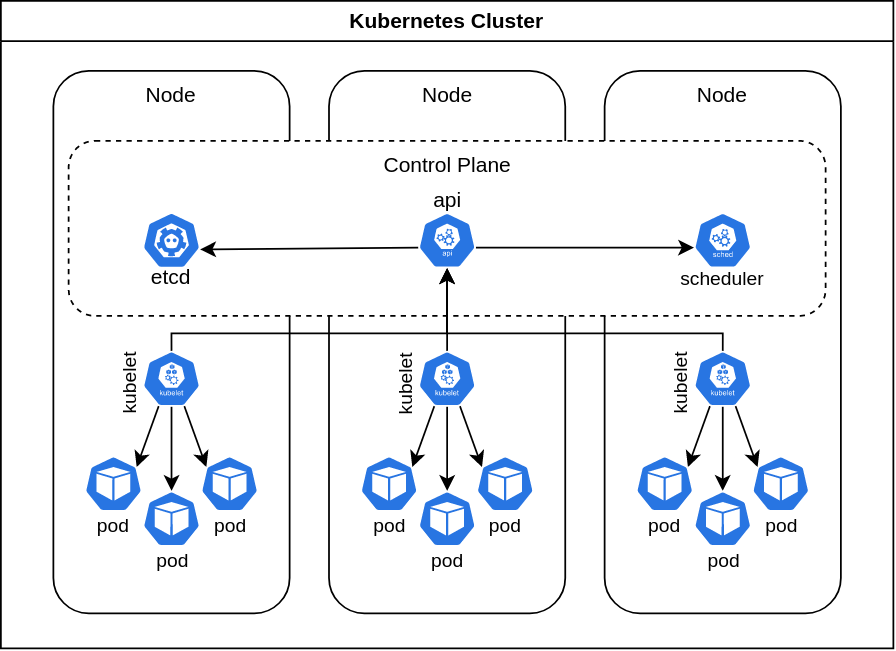
\includegraphics{resources/kubernetes-overview.png}
  \caption{A simplified overview over the Kubernetes components.}
  \label{fig:kubernetes-overview}
\end{figure}

\begin{description}
  \item[Nodes]
    (Possibly virtual) machines running containerized applications. On each node
    runs a component called kubelet that manages the pods and the corresponding
    containers on the node.
  \item[Pods]
    A group of containers that share storage and network resources that models
    an application-specific logical host. The containers that make up a pod are
    always located on the same node and are scheduled in unison.
  \item[Control Plane]
    A collection of pods that manage the nodes and workload pods inside the
    cluster. This includes an API, a backing store (etcd) for all cluster data,
    and a scheduler that assigns pods to nodes.
  \item[Container Runtime]
    Responsible for executing containers on a node (see section
    \ref{sec:container-runtime}).
\end{description}

\todo[inline]{Kubernetes: Expand as needed in the next chapters}

Kubernetes' non-monolithic design allows the replacement of almost every aspect
and component of a cluster. This allows a Kubernetes cluster to be run on
basically any underlying infrastructure, regardless of the hardware choices or
networking design.

There are three levels in a Kubernetes cluster on which confidentiality can be
applied to: The node, pod, or container. There are distinct benefits and
problems for applying confidentiality on each layer. We will discuss them in the
following sections.

\subsubsection{Confidential Nodes}

The most outer layer where confidentiality can be applied to in the Kubernetes
architecture are the nodes. By using confidential computing enabled virtual
machines -- for example by facilitating AMD SEV or Intel TDX -- a Kubernetes
cluster operator is able to shield workloads running inside the cluster.
Prominent service providers like Azure and GCP already offer the option of
deploying their managed Kubernetes clusters with confidential worker nodes.
However, these solutions do not include verification of the nodes which means
that one would have to build a custom remote attestation system -- for example
by implementing the RATS (section \ref{sec:rats}).

The biggest problem with confidential nodes is the restriction of cluster admin
privileges and verifying these as a client. While the workloads are shielded
from the infrastructure cluster administrators would still have full control
over the workloads running inside the cluster which breaks goal
\subGoalRef{2}{1}.

\subsubsection{Confidential Containers}

The other extreme would be to apply confidentiality to containers. A process
running inside a TEE would only receive confidential data like decryption keys
or personalized information after verifying that the process is running inside a
TEE via remote attestation. Since the TEE shields the process from the cluster
this approach remove the cluster administrator from the TCB of the application.

Even though this approach does not conflict with the goals of this paper, it does
collide with the design of Kubernetes. In the Kubernetes architecture the
smallest deployable unit of computation is a pod, a collection of application
containers. These containers share storage and network resources, but it becomes
very hard to share these resources when the containers are shielded from each
other. The next approach addresses this architectural issue.

\subsubsection{Confidential Pods}
\label{sec:confidential-applications}

Instead of applying confidentiality to containers we can also shield pods from
the outside world. This improves the last approach as per definition a pod in a
Kubernetes cluster defines an application-specific logical host. As opposed to
shielding a single container, shielding a pod would allow sharing storage and
networking resources between containers composing the pod.
